\documentclass{article}
\usepackage{todonotes}
\usepackage{tikz}
\usetikzlibrary{arrows,automata}

\usepackage[backend=bibtex,citestyle=authoryear,style=alphabetic,natbib]{biblatex}
\addbibresource{PaperTools/bibtex/jp.bib}
\addbibresource{phorae.bib}
\addbibresource{IWCSbib.bib}

\usepackage{stmaryrd}
\usepackage{newunicodechar}
\input{PaperTools/latex/newunicodedefs}

\title{FraCaS: 80 percent complete}

% - Two-phase system (Dyn semantics from theorem proving)
% - Anaphora (as in Jolli paper) --- but this is the first time that this is done for FraCas.
% - Multiple readings
% - Threshold-based interpretation of (some) adjectives + Linear arithmetic proofs
% - New handling of prepositions and adverbs
% - Definites handled by adding an assumption at the top-level. (instead as inline existential) -- Enabled by dyn. semantics
% - Plurals/Quantifiers improved
% - Genders are properties of nouns
% - Handling of comparatives (with threshold BUT not those of adjectives), relying largely on the dyn. semantic system

\begin{document}



\section{Introduction}

\paragraph{Contributions}
(see list above)
\section{Background}

\section{Overview of the system}

Our system consists of two main parts.
\begin{enumerate}
\item A converter from syntax trees to types. The syntax trees follow
  the GF formalism, and the types follow the Coq formalism. The
  converter itself is a Haskell program. It implements a dynamic
  semantics. It comprises the bigger part of our system.
\item A number of type-theoretical combinators. These take care of the
  natural semantics which have no influence on the dynamical
  aspects. This includes for example the treatment of adjectives
  (intersective, subsective, etc.) and adverbs (veridical or not).
\end{enumerate}
This architecture is represented schematically in Figure \ref{fig:overview}.

\begin{figure}
  \centering
{
  \tiny
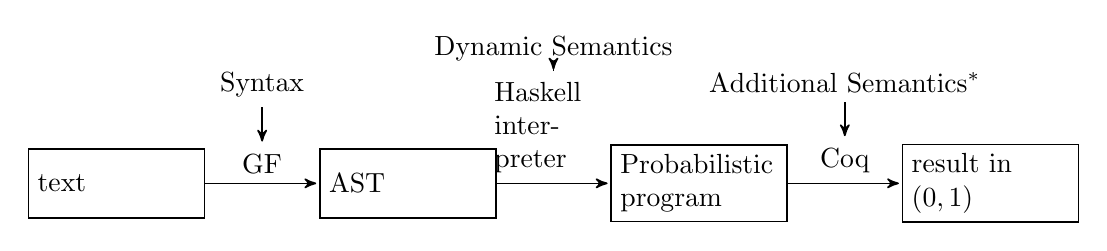
\begin{tikzpicture}[->,>=stealth',shorten >=1pt,auto,node distance=3.7cm,
                    semithick]
  \tikzstyle{every state}=[draw=black,text=black,shape=rectangle,text width=2cm]

  \node[state]         (txt)                {text};
  \node[state]         (ast) [right of=txt] {AST};
  \node[state]         (pp)  [right of=ast] {Probabilistic program};
  \node[state]         (res) [right of=pp] {result in $(0,1)$};

  \path (txt) edge              node (GF)  {GF}                  (ast)
        (ast) edge              node (Hask) [text width=1.5cm]{Haskell interpreter} (pp)
        (pp) edge               node (Coq) {Coq} (res);

  \node (Syntax) [above of=GF,node distance=1cm] {Syntax};
  \node (Sem) [above of=Hask,node distance=1cm] {Dynamic Semantics};
  \node (Hyper) [above of=Coq,node distance=1cm] {Additional Semantics$^\ast$};

  \path
  (Syntax) edge (GF)
  (Sem) edge (Hask)
  (Hyper) edge (Coq);
\end{tikzpicture}
}
\caption{Phases in our system. ($\ast$) At the level of Coq, we handle
  the details of the adverbial (veridicality properties) and
  adjectival semantics (division into subsective, extentional,
  non-committal, etc. categories.) }
  \label{fig:overview}
\end{figure}

All underlying systems (GF, Haskell, Coq) are based on lambda calculi
with types. We ensure that each translation preserve typing, locally:
\begin{enumerate}
\item Every GF syntactic category $C$ is mapped to a type noted $⟦C⟧$.
\item GF Functional types are mapped compositionally : $⟦A → B⟧ = ⟦A⟧ → ⟦B⟧$
\item Every GF syntactic construction function $f : X$ is mapped to a function $⟦f⟧$ such that $⟦f⟧ : ⟦X⟧$.
\item GF function applications are mapped compositionally: $⟦t(u)⟧ = ⟦t⟧ (⟦u⟧)$.
\end{enumerate}
Because all system embed the simply-typed lambda calculus, ensuring
type-preservation locally means that types are preserved globally.
Therefor, we are certain that every GF syntax tree can be mapped to
Haskell, and eventuall Coq, without error.

The dynamic semantics follows a monadic structure, as pioneered by
\citet{Shan:2002}. There are two kinds of effects carried by the
monad.  The first one comprises a series of state updates and queries,
corresponding to all elements that can be referred to by anaphoric
expressions. These can be usual ones (like NPs), but also less usual
ones (like 2-place verbs, or a quantity --- which we illustrate
below). The other kind of effects is \emph{non-determinism}. This
models the property that linguistic expressions can have several
interpretations. The monadic structure allows to locally express that
a given expression has several meaning; the monadic bind ensures that
all combinations of meanings are considered at the top-level,
combinatorially. This dynamic semantics allows us to model many
phenomena in a precise way:

\paragraph{anaphora} We can handle anaphora % wait so see what JoLLi says here

  % - Dynamic Semantics/Anaphora (as in Jolli paper) --- but this is the first time that this is done for FraCas.
%   -> Gender is a property of nouns
\paragraph{ellipsis} Ellipsis is handled in essentially the same way
as anaphora. This method is made especially straightforward thanks to
using GF syntax tree, which requires an explicit argument for each
predicate. Thus, ellpsis are made explicit by the parsing phase.

\paragraph{definites} A naive way to handle definites is as sigma (or
exsistential types). \todo{add example} However, if the semantics
does not feature a dynamic element, then the existential
quantification is introduced locally. This means that the quantifier
can be introduced in the wrong context. Consider the phrase
``everyone pets the dog''. The structure of the interpretation would
be be $∀x. person(x) → ∃y. dog(y) ∧ pet(x,y)$.

Instead, our take is that definites should be treated as anaphoric
expressions. If the referent is not found in the discourse, then it
will be introduced using a sigma type, \emph{at the top-level} of
the expression. Therefore we record all definites without referent,
using a monadic effect. When the complete sentence has been
interpreted, we re-introduced referent using existentials. For the
above example, we obtain the desired interpretation:
be be $∃y. dog(y) ∧ ∀x. person(x) → pet(x,y)$.

\paragraph{Phrasal comparatives}
Previous attempts to tackle section of the FraCaS test suite showed
that handling comparatives is not easy. Our strategy here is to
leverage our dynamic semantics, revealing an anaphoric element of
comparatives. Consider the hypothesis of FraCaS 239: ``ITEL won more
orders than APCOM lost.''  We postulate that this sentence is
equivalent to the following two separate parts: ``APCOM lost zero or
more orders. ITEL won more orders [than some elliptic quantity].''
The elliptic quantity is introduced every time we talk about some
quantity (indexed by a CN, in this case ``orders''), and it can be
referred to by a comparative, later in the discourse. Using this idea,
we can go one level deeper in the interpretation of our example:
``APCOM lost θ orders. θ >= 0.  ITEL won at least θ+1 orders.''. We
see here how the quantities are introduced. They are added to the
environment so that, they can be referred to as elliptic quantity
expressions. Finally, ``more'' is intepreted as ``at least <elliptic
quantity>+1''.


\paragraph{Adjectives}
In our system, we interpret gradable adjectives using a pair of a
measure $m : objects → Z$ and and a threshold $τ : Z$, where $Z$ is
treated as an abstract ordered ring by Coq. (This structure has no
dynamic aspect in our model, and thus is entirely handled within Coq.)
For subsective adjectives, $τ$ will additionally depend on the class
of the object in question. This structure has the benefit that
opposite adjectives can be easily represented (measures are opposites
$∀x. m_1 x = -m_2 x$ and thresholds do not overlap $τ_1 + τ_2 > 0$).
\todo{reference to this view in the litterature}.  Additionally,
adjectival assumptions as given in FraCaS are interpreted as linear
equations in $Z$. Because solving such equations is decidable, solving
such problems can be made efficient. Indeed, the tactic that Coq
offers for this purpose can solve all such problems in FraCaS,
automatically.


\paragraph{Adverbs}
Another point, of minor theoretical importance but major practical
one, is our handling of adverbial phrases. We interpret adverbs (and
in general all adverbial and prepositional phrases) are VP-modifiers:
$Adv = VP → VP$, where $VP = object → Prop$. However, applying
adverbs to verb-phrases heavily complicates the Coq proofs, because
such phrases can contain quantifiers. Therefore, we instead move the
adverbs, so that they apply to (atomic) verbs only, and can simplify
proofs accordingly. \todo{theoretical justification in the literature}



\section{Results and evaluation}

We evaluated FraCoq against 8 sections of the FraCaS test suite, for a
total of 259 examples. We excluded only one section, 7. The reason for
doing so is that, in our view, it contains too many examples which
require \textit{ad-hoc} treatment, and thus makes little sense to
include without complementing it with a more thorough suite which
captures a more complete landscape of the phenomena that section 7
touches.

FraCaS intends to classify each problem as either entailment (YES),
entailment of the opposite (NO) or no entailment (UNK).  For this
work, we have amended FraCaS to address a few problems. First, certain
test case are not formed correctly. Those were identified by Bill
MacCartney as ``undef'', and we removed those. Second, a few test
cases occurs twice in the suite, but with two different answers (one
YES and one UNK), with the annotation that those correspond to
different readings. However, elsewhere in the suite, if a problem has
several readings but only one has entailment, it occurs only once and
is marked as YES. To make the test suite consistent, if one reading
yields entailment we have always considered it as YES. Finally, we
have removed case 199 (which appears to be vacuous), and changed the
following cases, which appeared to have been misclassified. We note
that the majority of the mistaken classifications occur in sections 3
and 4, which have not been previously attempted and thus, we propose,
have not been properly scrutinized.

\begin{center}
\begin{tabular}{ccc}
 test case & new class & comment \\ \hline
    005 & UNK & missing hypothesis: there are italian tenors \\
   056 &  Yes & Already identified as such by MacCartney \\
  069 & Unk & Mary could have used someone else's workstation \\
  119 & Unk & \textit{ibid.} \\
  181 & Yes & for the same reason as 180 \\
  226 & Yes &
\end{tabular}
\end{center}

Our system classifies a case as YES if a proof can be constructed from
the premises to the hypothesis, NO if a proof of the negated
hypothesis can be constructed and UNK otherwise. Because we work with
a non-decidable logic, one can not \emph{in general} conclude
decisively that no proof exists. Thus, we consider here that no proof
exists if it cannot be constructed with reasonable effort. In
particular, we test at the minimum that the automatic proof search
built in Coq does not succeed before classifying a problem as UNK.


%  ------ Section 1
% complete: 74/74   []
% correct: 71/74   [13,14,46]
% score: 0.9594594594594594
%  ------ Section 2
% complete: 33/33   []
% correct: 27/33   [84,91,94,95,109,111]
% score: 0.8181818181818182
%  ------ Section 3
% complete: 27/28   [137]
% correct: 24/27   [124,126,127]
% score: 0.8571428571428571
%  ------ Section 4
% complete: 47/52   [171,172,191,193,195]
% correct: 45/47   [170,188]
% score: 0.8653846153846154
%  ------ Section 5
% complete: 20/20   []
% correct: 19/20   [216]
% score: 0.95
%  ------ Section 6
% complete: 29/31   [244,245]
% correct: 27/29   [242,250]
% score: 0.8709677419354839
%  ------ Section 7
% complete: 0/67   [251,252,253,254,255,258,259,260,261,262,263,264,265,266,267,268,269,270,271,272,273,274,275,277,278,279,280,281,282,283,284,285,286,287,288,289,290,292,293,294,295,296,297,298,299,300,301,302,303,304,306,307,311,312,313,314,315,316,317,318,319,320,321,322,323,324,325]
% correct: 0/0   []
% score: 0.0
%  ------ Section 8
% complete: 8/8   []
% correct: 6/8   [326,333]
% score: 0.75
%  ------ Section 9
% complete: 13/13   []
% correct: 12/13   [346]
% score: 0.9230769230769231
%  ------ Section 0
% complete: 251/259   [137,171,172,191,193,195,244,245]
% correct: 231/251   [13,14,46,84,91,94,95,109,111,124,126,127,170,188,216,242,250,326,333,346]
% score: 0.8918918918918919

\providecommand\forcecenter{\multicolumn{1}{c}}
\begin{table}
  \centering
\begin{tabular}{rlrrrrrr}
  & Section      & \# examples & Ours     & FraCoq & MINE & Nut  & Langpro  \\ \hline
1 & Quantifiers  & 75          & .96 (74) & .96    & .77  & .53  & .93 (44) \\
2 & Plurals      & 33          & .82      & .76    & .67  & .52  & .73 (24) \\
3 & Anaphora     & 28          & .86      &   -    & -    & -    &  -       \\
4 & Ellipsis     & 52          & .87      &   -    & -    & -    &  -       \\
5 & Adjectives   & 22          & .95 (20) & .95    & .68  & .32  & .73 (12) \\
6 & Comparatives & 31          & .87      & .56    & .48  & .45  &  -       \\
8 & Verbs        & 8           & .75      &   -    & -    & -    &  -       \\
9 & Attitudes    & 13          & .92      & .85    & .77  & .46  & .92 (9)  \\ \hline
  & Total        & 262         & .89      & .83    & .69  & .50  & .85  \\
  &              &             & (259)    & (174)  & (174)& (174)& (89)
  \end{tabular}
  \caption{Overview of the accuracy of our system compared to others.
    ``Ours" refers to the approach presented in this paper. When a
    system does not handle the nominal number of examples shown in the
    third column, the actual number of examples attempted is shown in
    parentheses.  ``FraCoq'' refers to the work of
    \citet{bernardy_type_2017}. ``MINE" refers to the approach of
    \citet{Mineshima:2015}, ``NUT" to the CCG system that utilizes the
    first-order automated theorem prover \textit{nutcracker} described
    by \citet{bos:2008}, and ``Langpro" to the system presented by
    \citet{Abzianidze:2015}.  }
\end{table}


The above result reveals a considerable improvement over earlier
approaches in terms of coverage, with three more sections covered over
previous state of the art. Additionally, our system is generally best
in terms of accuracy overall. In particular, section 6 sees a large
improvement in accuracy, which we attribute to our new analysis of
comparatives, enabled by our dynamic semantics.

\paragraph{error analysis}
Our system fails to classify correctly 28 problems of of 259 attempts.
Unfortunately, it isn't easy to concisely characterize the areas where
it fails.  The biggest source of error can be attributed to its
incorrect handling of groups
(013,014,046,084,111,124,126,127,137,171,172,191,193,195,243,250,333,346). These
are cases where a conjunction of individuals is treated as group, or
where counting members of a group is necessary.  Other notable
problematic cases are that definite plural does not have universal
reading are incorrectly classified (091,094,095). Neither measure
phrases (242) nor attributive comparatives (244,245) are handled.


\section{Future work}
\section{Conclusion}


\printbibliography

\end{document}